\chapter{Desarrollo realizado}

En el momento actual están realizadas las siguientes aplicaciones

\section{Base de datos de accesos}
Se encuentra finalizada, pero todavía es susceptible a cambios. Se ha implementado sobre SQLite debido a la sencillez y a que el SQL empleado es bastante estándar (sería sencillo pasarla a otro sistema de gestión de bases de datos).

\section{Interfaz de Gestión de accesos}
Se encuentra en estado Beta. Falta por finalizar la parte referente a listados, mejorar los temas de configuración y de tratamiento de errores, diálogos de "Acerca de" y pulir detalles al respecto.

\begin{figure}[h!]
        \centering
        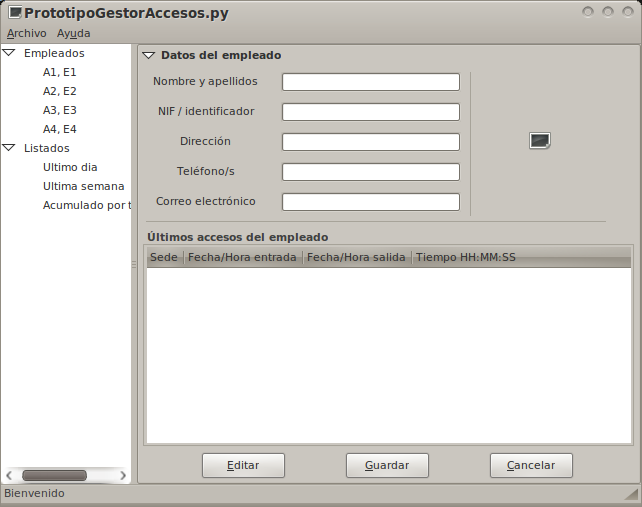
\includegraphics[width=8cm]{PrototipoGestorAccesos.png}
        \caption{Interfaz de gestión de accesos (prototipo)}
	\label{fig:gestion_accesos}
\end{figure}


\section{Base de datos biométricos}
Tras una toma de estadísticas y la consideración de cuál es el mejor método de almacenamiento de datos para las huellas faciales, se procederá a la creación de la base de datos biométricos.

\section{Interfaz de Reconocimiento}
Actualmente se encuentra en estado beta. Faltan por pulir detalles en cuanto a diálogos de configuración, tratamiento de errores y diálogos de "Acerca de".

\begin{figure}[h!]
        \centering
        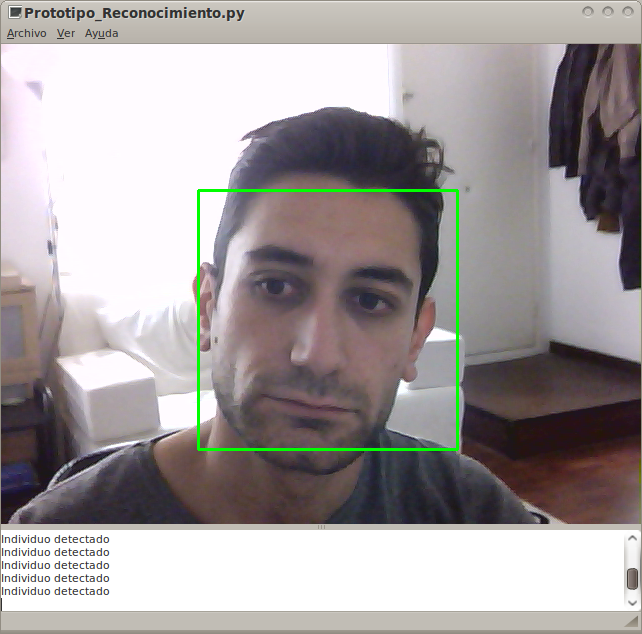
\includegraphics[width=8cm]{PrototipoReconocimiento.png}
        \caption{Interfaz de Reconocimiento (prototipo)}
	\label{fig:reconocimiento}
\end{figure}

\section{Interfaz de Captura}
Todavía no disponible. En cuanto se haya determinado el mejor método para almacenar los datos biométricos, se iniciará.
